\documentclass[tikz,border=2pt]{standalone}
\usepackage{unicode-math}
\setmainfont[
  Path=publication/fonts/,
  UprightFont=source-serif-4-latin-400-normal.ttf,
  ItalicFont=source-serif-4-latin-400-italic.ttf,
  BoldFont=source-serif-4-latin-600-normal.ttf,
  BoldItalicFont=source-serif-4-latin-600-italic.ttf
]{Source Serif 4}
\setmathfont[Path=/System/Library/Fonts/Supplemental/]{STIXTwoMath.otf}
\usepackage{tikz}
\usetikzlibrary{arrows.meta,backgrounds,calc,decorations.pathreplacing,fit,matrix,positioning}
\definecolor{BookInk}{HTML}{18232D}
\definecolor{BookBlue}{HTML}{315F78}
\definecolor{BookRed}{HTML}{98452F}
\definecolor{BookGreen}{HTML}{3F6659}
\definecolor{BookMuted}{HTML}{66727A}
\definecolor{BookRule}{HTML}{AEB7BC}
\tikzset{
  book/node/.style={
    draw=BookInk, line width=.55pt, fill=white,
    minimum height=9mm, inner xsep=5pt, inner ysep=4pt,
    font=\footnotesize, align=center
  },
  book/primary/.style={book/node, draw=BookBlue},
  book/decision/.style={book/node, draw=BookRed},
  book/verified/.style={book/node, draw=BookGreen},
  book/arrow/.style={
    -{Stealth[length=2mm,width=1.35mm]}, line width=.55pt, draw=BookInk
  },
  book/quietarrow/.style={
    -{Stealth[length=2mm,width=1.35mm]}, line width=.45pt, draw=BookRule
  },
  book/feedback/.style={
    -{Stealth[length=2mm,width=1.35mm]}, line width=.5pt,
    draw=BookRed, dashed
  },
  book/note/.style={font=\scriptsize, text=BookMuted, align=center}
}

\begin{document}
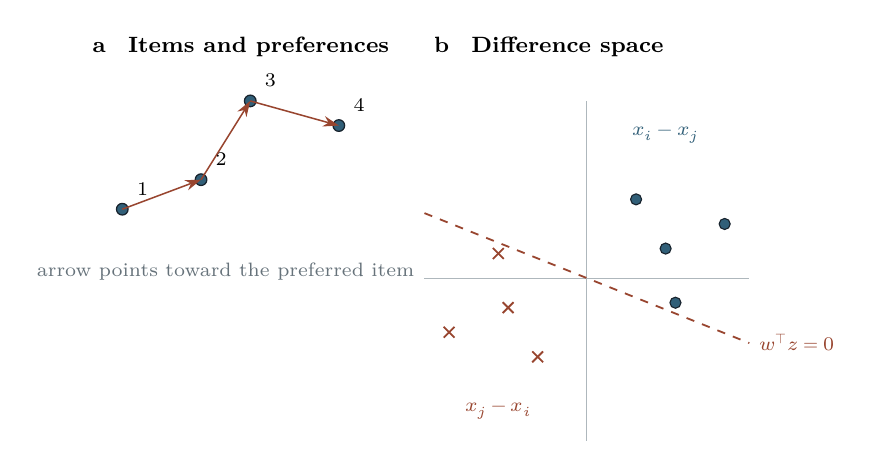
\begin{tikzpicture}[x=1.25cm,y=1.25cm]
  \begin{scope}
    \node[font=\footnotesize\bfseries,anchor=west] at (0,2.35) {a\quad Items and preferences};
    \foreach \x/\y/\n in {.4/.7/1,1.2/1/2,1.7/1.8/3,2.6/1.55/4}{
      \filldraw[fill=BookBlue,draw=BookInk,line width=.45pt] (\x,\y) circle (2.1pt);
      \node[font=\scriptsize,anchor=south west] at (\x+.05,\y+.04) {\n};
    }
    \draw[book/arrow,draw=BookRed] (1.7,1.8)--(2.6,1.55);
    \draw[book/arrow,draw=BookRed] (1.2,1)--(1.7,1.8);
    \draw[book/arrow,draw=BookRed] (.4,.7)--(1.2,1);
    \node[book/note,anchor=north] at (1.45,.25) {arrow points toward the preferred item};
  \end{scope}
  \begin{scope}[xshift=6.4cm]
    \node[font=\footnotesize\bfseries,anchor=west] at (-1.65,2.35) {b\quad Difference space};
    \draw[BookRule] (-1.65,0)--(1.65,0);
    \draw[BookRule] (0,-1.65)--(0,1.8);
    \draw[BookRed,dashed,line width=.65pt] (-1.65,.66)--(1.65,-.66)
      node[anchor=west,text=BookRed,font=\scriptsize] {$w^\top z=0$};
    \foreach \x/\y in {.9/-.25,.5/.8,.8/.3,1.4/.55}{
      \filldraw[fill=BookBlue,draw=BookInk,line width=.4pt] (\x,\y) circle (2pt);
      \draw[BookRed,line width=.65pt] (-\x-.055,-\y-.055)--(-\x+.055,-\y+.055);
      \draw[BookRed,line width=.65pt] (-\x-.055,-\y+.055)--(-\x+.055,-\y-.055);
    }
    \node[book/note,text=BookBlue] at (.8,1.45) {$x_i-x_j$};
    \node[book/note,text=BookRed] at (-.9,-1.35) {$x_j-x_i$};
  \end{scope}
\end{tikzpicture}
\end{document}
